%-------------------------------------------------------------------------------
\section{Data Disguising}
%-------------------------------------------------------------------------------
\iffalse
\begin{figure}[t!]
    \centering
    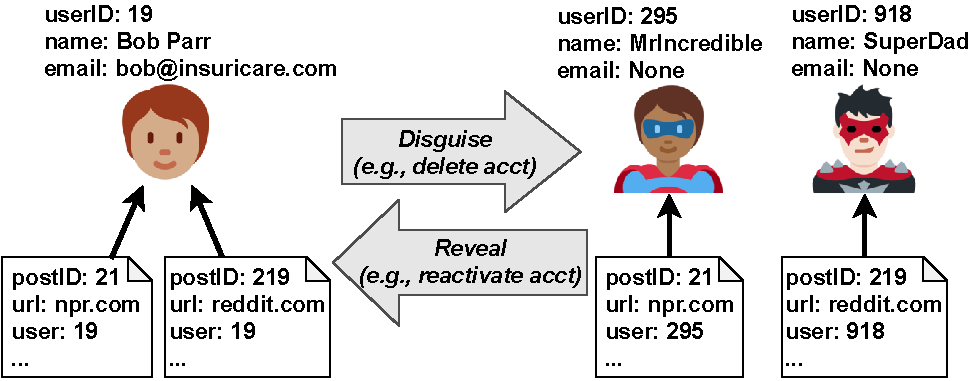
\includegraphics[width=0.5\textwidth]{img/disguises}

    \caption{Disguises move the target object (in this example, a user Bob) from an identity-revealing
    guise to privacy-preserving guises.}
    \label{fig:example}
\end{figure}
\fi

\begin{figure*}[t!]
    \centering
    \footnotesize
\begin{tabular}{@{}c|c|c|c@{}}
\textbf{User Transformation Spec} & \textbf{User Object} & \textbf{Guise 1} &
    \textbf{Guise 2} \\
\begin{lstlisting}[language=Rust]
"id":       IDAttribute,
"name":     Gen(Random),
"active":   Gen(Default(false)),
"darkmode": CopyAll,
"notifs":   CopyOnce+Gen(Default(false)),
"tag_id":   GenForeignKey,
\end{lstlisting}
    &
\begin{lstlisting}[language=Rust]
"id":       19,
"name":     BobParr,
"active":   true,
"darkmode": false,
"notifs":   true,
"tag_id":   11
\end{lstlisting}
&
\begin{lstlisting}[language=Rust]
"id":       295,
"name":     MrIncredible,
"active":   false,
"darkmode": false,
"notifs":   true,
"tag_id":   81483
\end{lstlisting}
&
\begin{lstlisting}[language=Rust]
"id":       918,
"name":     SuperDad,
"active":   false,
"darkmode": false,
"notifs":   false,
"tag_id":   15592
\end{lstlisting}
\end{tabular}
    \caption{Creating two guises of an example user (of a synthetic application schema).}
    \label{fig:guises}
\end{figure*}



The key idea behind \emph{data disguising} is to associate multiple \emph{guises} with a target
data object. Guises vary in how they reveal identities or preserve privacy.
%
Objects move between different guises by means of privacy transformations.
%
%Figure~\ref{fig:example} illustrates this with the example of user account deletion.
%
When his account is active, user Bob's profile is associated with his true identity and all his
contributions to the site (an identity-revealing guise).
%
When Bob deletes his account, his profile and contributions move to different, privacy-preserving
guises: his name has been anonymized, his email address has been redacted, and his contributions
have been decorrelated and attributed to individual, unidentified user guises.
%

%
Data disguising builds on the existing structure of web applications.
%
Web applications are often structured as object graphs, either explicitly~\cite{tao, delf},
through an object-relational model (ORM)~\cite{orm}, or implicitly via foreign keys (edges)
between tables (vertices) in relational databases.
%
Data disguises transform this object graph.
%

%
The application developer writes a disguise specification for each privacy transformation needed
in the application.
%
This specification is a declarative statement similar to a relational schema, with entries for
graph vertices (objects) and directed edges (relationships between pairs of objects)
to be transformed (see \S\ref{sec:policies}).
%
We assume that:
\begin{enumerate}[nosep]
  \item developers use their domain knowledge to write correct and complete disguises;
  \item application code handles the different guises appropriately (\eg in
    displaying them); and
  \item different guises of the same object have the same structure (\eg they can be
    rows in the same table).
\end{enumerate}
%
A data disguising tool takes the disguise specification and turns it into storage operations that
apply the transformation (disguise) or its reverse (reveal).
%
At any given moment, an application's data object graph comprises a mix of
identity-revealing guises and privacy-preserving ones. Privacy transformations split
and combine individual guises when triggered.

%-------------------------------------------------------------------------------
\section{Specifying Data Disguises}
%-------------------------------------------------------------------------------
\label{sec:policies}

A data disguise is written once by the developer, and applied in the context of a specific target
object to disguise, such as a departing user, and a specific instance of he object graph.
%
The disguise consists of context-specific transformations that turn objects into one or
more guises (or remove the object completely). 
%Developers specify disguises in two parts. The
%first specifies how to create guises of a given object type (\S\ref{sec:guises}). The second specifies in which
%contexts objects should be transformed into guises or removed (\S\ref{sec:context}).
%
A disguising tool then applies the disguise by first determining the current context of objects in the object
graph, and then applying the appropriate transformation for that context.
%\ie from what type of edge, and sensitivity context.

\subsection{Context-Specific Transformations}
\label{sec:context}

Developers specify \textbf{contexts}, and transformations to the objects that match each context. 
%
% SOURCE = CHILD
% DEST = PARENT
%
%In the following, we refer to edge types in the object graph, which have a \emph{source} object type and a \emph{destination} object type,
%where the source references the destination (\eg via a foreign key column in a relational database).
%
A context consists of an object type, and a set of constraints on the objects' attributes
(\S\ref{sec:constraints}).
Given an instance of the object graph, a set of objects in the graph
satisfy the context if the objects are of the specified object type and the objects'
attributes satisfy the constraints.

For each context, developers specify to either remove matching objects (which also removes all
descendents---objects that refer to these objects---as well), or to transform each object into
a single guise (\S\ref{sec:single_guise}). 

%
In the following, we assume that objects have identifier attributes (\eg \texttt{id} in Figure~\ref{fig:guises}); and
some attributes are reference attributes that form edges in the graph to referred objects (\eg
\texttt{tag\_id} is a foreign key constraint to tag objects).

\subsection{Object Attribute Constraints}
\label{sec:constraints} 

Object attribute constraints consist of (some conjunction) of the following constraints:
\begin{itemize}[nosep]
\item \textbf{Reference content} constraints on reference attributes are functions that
    take both the object and the referenced object as input, and return true or false. 
    %
    %For example, perhaps we want to decorrelate paper-tag edge \emph{only if} the tags were created by the user who is leaving.
\item \textbf{Value content} constraints on non-reference (value) attributes are functions that take the object as
input, and return true or false.  
\item \textbf{Sensitive reference} constraints on reference attributes match only objects that refer
    to sensitive objects (\ie connects back to the target object of the disguise).
\end{itemize}

\subsection{Single-Guise Transformations}
\label{sec:single_guise} 
Single-guise transformations are specified at attribute-level granularity. 
Guise identifier attributes are unique and random values. 
%
Other guise attributes either copy the original object attribute value, 
or transform the object attribute.  

If the attribute is a non-referencing, value attribute, the attribute transformation takes the
object attribute value as input, and generates a new guise value (\eg hashing the value, generating
random values, or setting the value to some default).  The guise attribute value depends at most on
the value of the object's attribute.

If the attribute is a reference attribute, the attribute transformation \emph{decorrelates} the 
object from the reference. Decorrelation creates a new reference guise based on the referenced
object (\S\ref{sec:reference_guises}), and the guise's reference attribute will refer to the
created reference.

\subsection{Reference Guise Creation}
\label{sec:reference_guises} 
%
Decorrelating references requires creating guises for the referenced objects. One referenced object may turn into many
reference guises (one for each context-matching object that all should be decorrelated).  Because
multiple reference guises may be created to decorrelate objects from the reference object,
developers needs to specify how to transform the reference object into a guise \emph{for each guise
created}.

%
Developers specify \textbf{many-guise transformations} for each object type that may be a reference;
these transformations are \emph{independent} of any single context, because many-guise
transformations only occur for the purpose of decorrelation, and can occur in many contexts.
%
Figure~\ref{fig:guises} shows an example, producing guises for user objects.

A many-guise transformation for an object type consists of a single-guise transformation (as
described above, \ie copying or generating new object attributes); and additional per-attribute
annotations that specify whether the transformation should be applied to create all guises, or
applied to create all but $n$ guises. In the latter case, $n$ guises will simply copy the
object's attributes, and the other guises will transform the object's attributes according to the
single-guise transformation.

Note that creating reference object guises may also require recursively creating guises for references of
the reference object, using the (context-independent) many-guise transformation for those ancestral reference
object types.

\subsection{Partially Applying Context Transformations}
\label{sec:threshold} 

Developers may want to transform some attributes in only a subset of all context-matching objects when
changing them into guises. 
For example, let the context match only the papers written by the targeted user. These papers should
be decorrelated from a tag only enough to ensure that these sensitive papers comprise less than 10\%
of all papers with that tag. Importantly, papers falling below the 10\% threshold can retain the
reference to the tag.

To transform attributes in only a subset of context-matching objects, developers can associate a
\emph{threshold} with an attribute of the context's object type.  A threshold is defined as follows:

Consider all objects of the context's object type that share the same attribute value (\eg a
referenced tag, or location value). This set contains both context-matching objects, and objects
ouside the context. The threshold for the attribute determines the maximum proportion of these
objects that are context-matching, and whose attribute value should not be transformed when the
object becomes a guise.

All context-matching objects falling above the threshold transform the attribute according to the
associated attribute transformation, while all objects falling below the threshold leave the
attribute unchanged. 

In our paper-tag example, the developer specifies a threshold of 10\% for the tag reference
attribute: any sensitive papers falling below the 10\% threshold can retain their reference to the tag.

Thresholds can also be associated with a set of
attributes, for example determining the maximum proportion of papers referencing a particular tag
\emph{and} a particular location attribute value that can match the context.

%same attribute(s), see k-anonymity?
%Figure~\ref{fig:algo} illustrates a constraint that sets a threshold (0.5) for the
%maximum proportion of papers connected to a tag that a targer-user's papers can make up.
%Because the target user's papers make up more than 0.5 of all papers connected to the tag,
%\sys decorrelates the sensitive paper sources from the tag until the user's papers fall
%below or at the threshold.
%%
%If the threshold is negative, then \sys decorrelates or deletes \emph{all} sources of that
%destination, including sources that were not traversed from the target object.

\lyt{TODO: What if context matches after you transform objects? (infinitely matching contexts?)}

\iffalse
\subsection{An Example Disguise}
\label{design:eg}
%
Consider disguising Bob when he deletes his HotCRP account.
%
Bob would prefer his papers and reviews to be unlinked from his identity.
%
HotCRP, on the other hand, would like to retain paper and review information that other users
find useful.
%
A careful selection of edge and object transformations achieves both.
%

%
To decorrelate reviews from Bob, the disguise \texttt{Decorrelate}s user-to-review edges.
%
This requires transforming Bob into one unique user guise per review.
%
The disguise generates guise attribute values using suitable defaults;
%
in particular, HotCRP users' \texttt{disabled} attribute is set for the guises,
ensuring that guises have no permissions and never review papers.
%

%
Bob is further linked to papers through conflicts, which can indicate coauthorship or a
reviewer conflict.
%
These conflicts are not reassigned to the new guises, since preserved
conflicts could reidentify Bob as the likely author of a review. Thus, the
conflict edges that link a disguised user to papers need a \texttt{Delete} annotation.
%
%% Edge directionality matters here: paper-to-conflict edges should not be removed, as doing so
%% could incorrectly allow conflicted users to see the paper!

The disguise \texttt{Retain}s all other edge types, ensuring that review and paper
artifacts remain correctly linked. Active reviewers still see the correct paper for their reviews,
and active authors see the correct reviews for their papers, albeit potentially authored by
anonymous, unlinkable guises of the original reviewer.
%
%Review and paper guises copy the original object, retaining paper and review information.
%
%\ms{Does this mean duplicate papers/reviews can show up?}

%
Unlike the current real-world HotCRP account deletion policy~\cite{hotcrp:privacy}, which
deletes all objects belonging to Bob, this disguise strikes a balance between decorrelating
Bob's identity from his reviews and papers, and maintaining useful information for other
HotCRP users.
%
Furthermore, it is easy to imagine extending this disguise to automatically disguise Bob
after some time (\eg 2 years after the conference), protecting his future research career
by hiding youthful reviewing sins.
\fi
